

\chapter{Reactive Programming}
Un sistema reattivo è un sistema \textit{event-driven} che interagisce continuamente con l'ambiente reagendo agli stimoli che da esso gli pervengono.\\
Si assume che i sistemi reattivi:
\begin{itemize}
	\item eseguono con una velocità mai sopraffatta da quella dell'ambiente;
	\item usualmente non terminino mai e quindi siano facilmente caratterizzabili da semplici funzioni che partendo da uno stato iniziale li portino ad uno stato finale.
\end{itemize}
I principi su cui si basa la \textit{reactive programming} sono i seguenti:
\begin{itemize}
	\item \textbf{Responsive:} il sistema deve rispondere ad una richiesta nel minor tempo possibile. Inoltre, con \textit{responsive} si intende anche individuare in maniera rapida un problema e trattarlo in modo efficace;
	\item \textbf{Resilient:} il sistema deve essere \textit{responsive} anche di fronte ad un errore. Ogni sistema non \textit{resilient} è anche non \textit{responsive} nel gestire gli errori;
	\item \textbf{Elastic:} il sistema deve restare \textit{responsive} anche all'aumentare del carico di lavoro. Questo implica che il sistema deve essere scalabile di fronte all'aumento della richiesta senza alcun cambiamento a livello di design del sistema;
	\item \textbf{Message-Driven:} i sistemi \textit{reactive} seguono il modello di programmazione asincrona, ottimizzando l'utilizzando delle proprie risorse.
\end{itemize}
\begin{figure}[h]
\centering
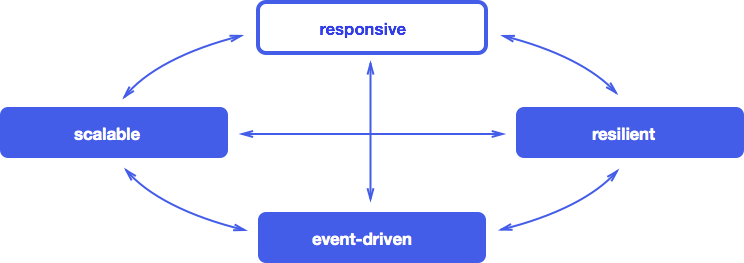
\includegraphics[width=0.7\linewidth]{immagini/react}
\caption[Rappresentazione del modello Reactive Programming]{Rappresentazione del modello Reactive Programming}
\label{fig:react}
\end{figure}

